\section{Data Collection and Basic Analysis}
\label{sec:data}


\begin{table}[h!]
\centering
\footnotesize
{
\begin{tabular}{l|l}
\hline
Metadata Field & Explanation \\
\hline                            
%\cline{1-1}
{\bf name}      & submitted file name \\
{\bf link}      & where to download the file \\
{\bf timestamp} & timestamp when the submission was made \\
{\bf source\_country} & the country where the submission was made \\
{\bf source\_id} & user ID who made the submission\\
{\bf size} & file size \\
{\bf type} & file type \\
{\bf tags} & labels with more specific information for each {\bf type}\\
{\bf first\_seen} & when the same file was first submitted \\
{\bf last\_seen} & when the same file was last submitted \\
{\bf hashes} & sha1, sha256, md5, and vhash\\
{\bf ssdeep} & ssdeep digest string \\
{\bf total} & number of engines analyzing the file \\
{\bf positives} & number of engines that flagged the file as malicious \\
{\bf positives\_delta} & changes in {\bf positives} across different submissions\\
{\bf report} & detailed detection report from each AV engine \\
\hline
\end{tabular}
}
\caption{VirusTotal Metadata. 
%\footnotesize{
(Fields for each submission retrieved from VirusTotal through distribution API and their related explanation.
One file could be submitted multiple times by different users.)
%}
}
\label{tab:fields}
\end{table}



This section introduces \vt{} and how we collect data from \vt{}. 
We also conduct simple analysis to understand 
the basic properties of our collected data. 

\subsection{\vt{}}
\vt{} is a free online malware scanning service. 
It was founded in 2004 and was acquired by google in 2012. 
\vt{} is widely used by anti-virus vendors to identify false positives and false negatives 
in their products~\cite{huangvt2016bigdata, neeles}, 
and individual users, including many academic people, 
as we discussed in Section~\ref{sec:label}.



For each submitted sample, \vt{} applies a set of anti-virus engines to analyze it. 
\vt{} keeps information about whether the submission is labeled as malware by each engine, 
and detailed tags for identified malware from each engine. 
\vt{} provides open APIs for users to interact with \vt{} 
and access the metadata of all submissions and latest detection results.
For example, \texttt{rescan} api asks \vt{} to analyze a previously submitted file again. 
\texttt{report} api returns detailed metadata and latest 
detection results for a file as shown in Table~\ref{tab:fields}. 
\texttt{distribution} api works like a pipe and keeps 
downloading information for latest submitted data from \vt{}. 

\subsection{Data Collection}

We started our data collection on August 31th, 2018. 
We randomly sampled 14423 PE files that was firstly submitted to \vt{} 
on that day using \texttt{distribution} api.
The reason we focus on PE files is that there are more 
than half \vt{} submissions are PE files~\cite{SongAPsys2016}. 
We control our sample to have roughly 
half files labeled as benign by all vendors 
and the left half labeled as malicious by at least one vendor.
We schedule a \texttt{rescan}, and then we use \texttt{report} API to acquire
the latest detection results every day after August 31th. 
We query \texttt{report} api two hours after the scheduled \texttt{rescan} to give 
\vt{} enough time to finish the rescanning analysis. 

Our data collection still continues. 
To write this paper, we use data from August 31th, 2018 to 
November 13th, 2018 to conduct experiments in future sections. 
In total, we use data collected in consecutive 75 days. 

\subsection{Basic Properties}


We conduct a set of analysis 
to learn various basic properties of our collected data.
These properties give an overview of how data set looks like
and serve as the foundation for our more 
advanced analysis in the next three sections. 

\noindent{\underline{File Properties.}}
All our sampled PE files are in 32 bit. 
Among them, 5798 are Win32 DLL files, 
and 8625 are Win32 EXE files.
For file size, more than 95\% sampled 
files are in the range from 4KB to 4MB. 
The smallest sampled file is only 800B, 
and the largest one is larger than 389MB.


\subsection{What information can we get from VirusTotal?}% I mean the data format. 


\subsection{Basic properties of the data set}

Now we take a look at the data set. First, there are 7197 malicious files and 7226 benign files according to the results from first scan. We say ``malicious'' as long as there is one vendor reporting malicious. This indicates that our dataset is balanced.

Then we check the completeness of the dataset by observing two distributions. 
Our dataset could be regarded as a set of tuples $(f, v, t)$ that sample $f$ is scanned at time $t$ by vendor $v$. Ideally, there should be one tuple for all $f, v, $ and $t$ in all 14423 files, more than 70 vendors and 75 days. 
However, not all valid tuples exist in the downloaded information. Some tuples may miss because of VirusTotal or our crawling configuration. So we calculated two distributions of the data set to check the completeness.
First, Figure~\ref{fig:dataset_submission_vendor_distri} shows the distribution of how many vendors have scanned a sample in a detection result. A point $(x, y)$ on the curve represents that there are $y$ detection results with $x$ vendors scanned. From the chart, we can know that most of the detection results are detected by more than 65 vendors. 
In addition, Figure~\ref{fig:dataset_no_vendors_scanned_moste_files_in_x_days} shows  how many vendors scan most of the files in how many days. More specifically, $(x, y)$ in the chart represents there are $y$ vendors that scans more than 90\% of the total files in $x$ days. The figure indicates that most of the vendors 
From the two figures, we could conclude that the dataset is mostly complete.

\begin{figure}
\centering
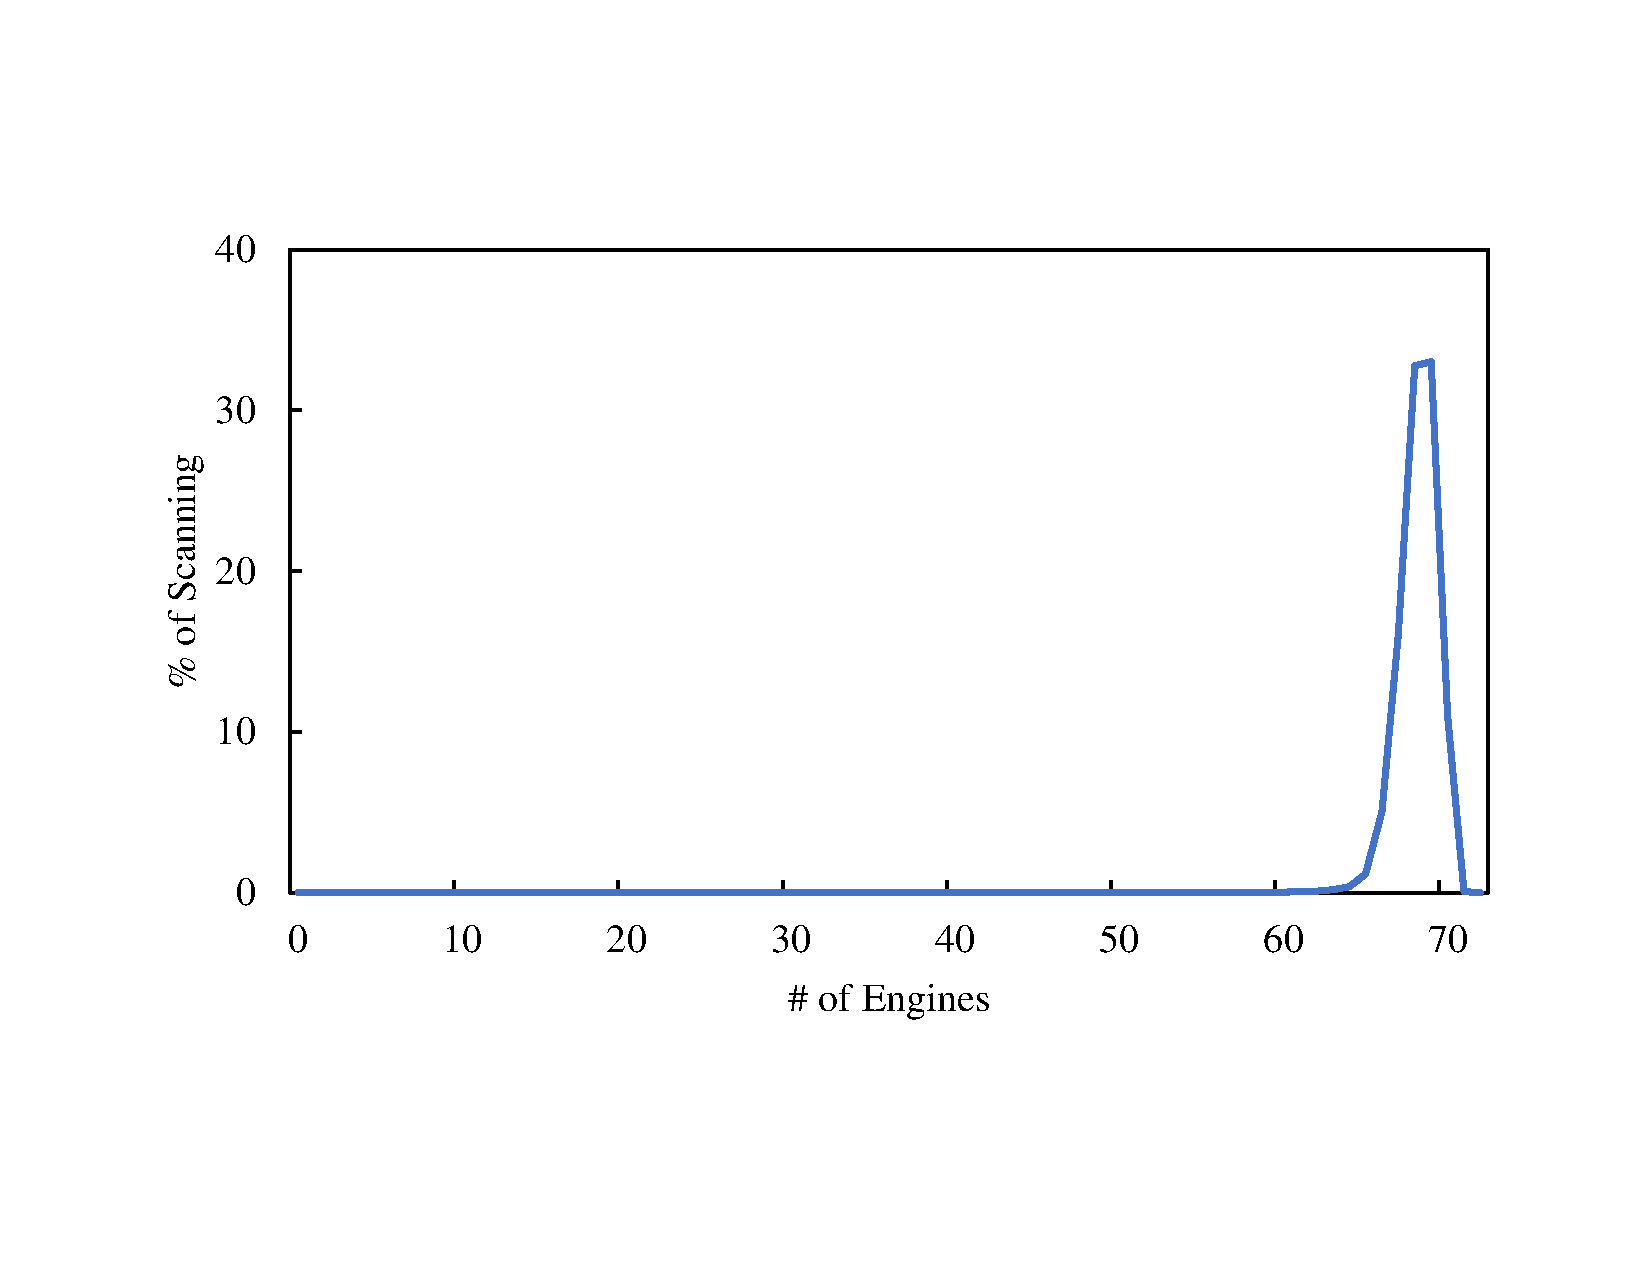
\includegraphics[width=0.7\linewidth]{figure/vendor_submission_distribution}
\caption{Distribution of detection results vs. vendors}
\label{fig:dataset_submission_vendor_distri}
\end{figure}

\begin{figure}
\centering
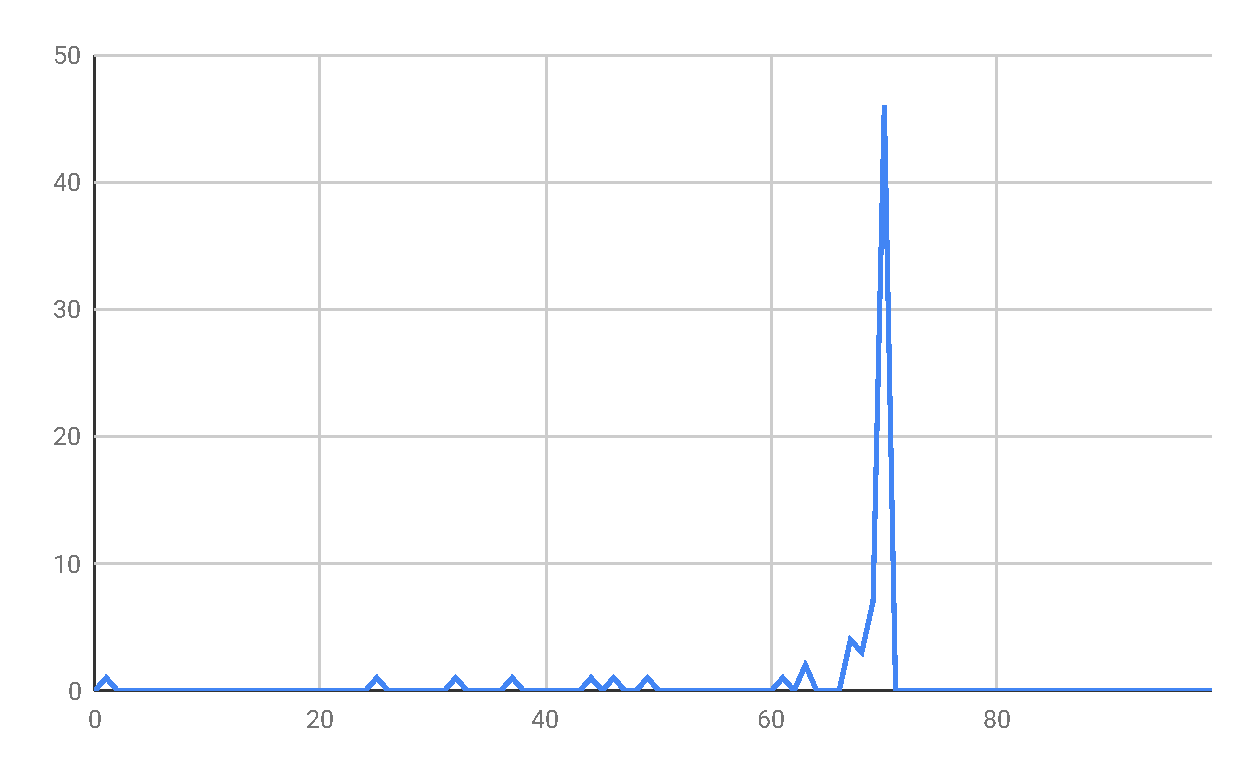
\includegraphics[width=0.7\linewidth]{figure/dataset_no_vendors_scanned_moste_files_in_x_days}
\caption{the number of vendors that scanned more than 12980 (>90\%) files in $x$ days}
\label{fig:dataset_no_vendors_scanned_moste_files_in_x_days}
\end{figure}


\subsection{How VirusTotal update engines?}
As we mentioned above, we use \texttt{rescan} and \texttt{report} to get the latest detection results from VirusTotal for each day. Actually, how VirtusTotal update the antivirus engines? With our data set for 75 days, we first check whether antivirus bases and versions update over time. We find that more than 78\% of the detection results updates consistently with time went on. So we can get new detection results from VirusTotal when we \texttt{rescan} samples and \texttt{report} detction results 2 hours later.


\begin{figure}
\centering
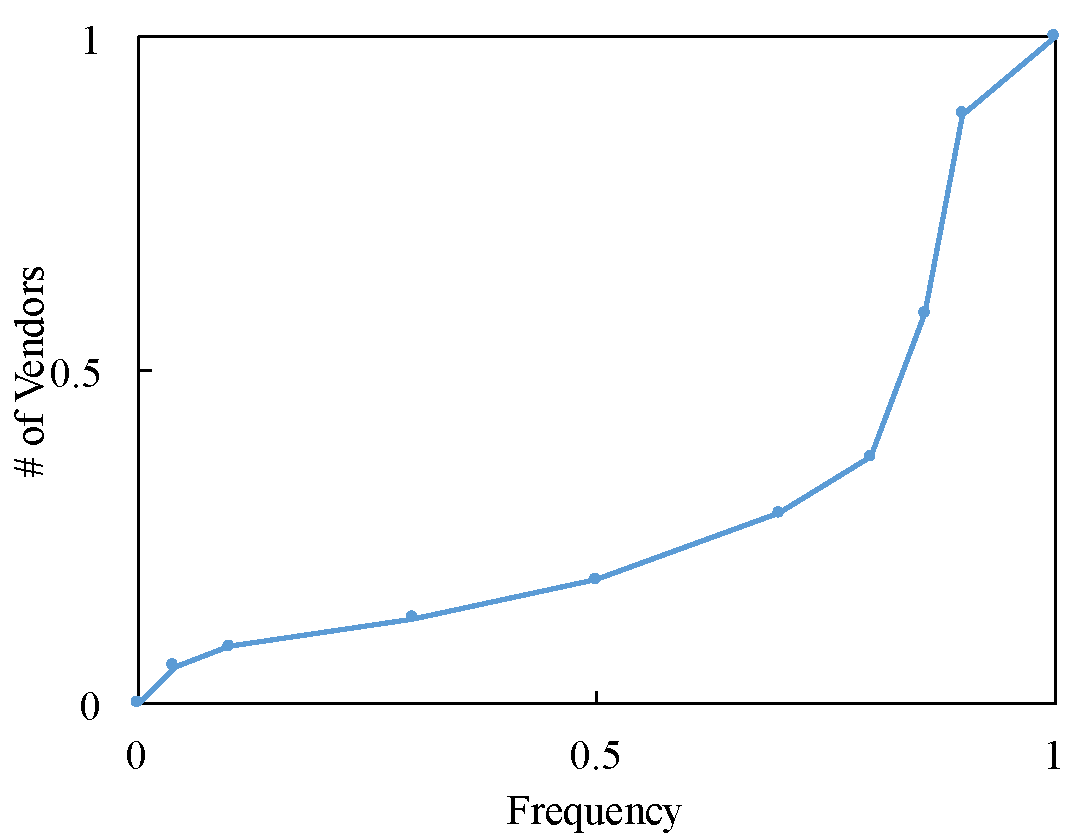
\includegraphics[width=0.7\linewidth]{figure/frequency}
\caption{Distribution of update frequency over vendors.}
\label{fig:frequency}
\end{figure}

Figure \ref{fig:requency} presents the distribution of updating frequency for vendors. Overall, more than 44 vendors(total 70) update their detction results with at least 1 day. Only 6 vendors' updating frequency are less than 0.05, and 4 of them seems not change their antivirus engines during these 75 days. Averagely, about 56 vendors will be updated with at least 2 days. 

%c. How VirusTotal update engines? Scanning time vs. update vs. version 
%TODO: need more data
\subsection{Caveats}

Discuss errors during our data collection. 
